\chapter{Event reconstruction}
\label{ch:reconstruction}

As described in Chapter~\ref{ch:lhcAndCMS}, the CMS detector
is built from complementary detector components with sensitivity
to stable particles: electrons, muons, photons, and charged
and neutral hadrons. Each can be distinguished by their likelihood of interaction
and interaction characteristics with the detector components:
all charged particles leave tracks in the inner tracker,
charged hadrons deposit energy in the calorimeters, photons
and electrons primarily deposit energy in the ECAL, and neutral
hadrons interact primarily with the HCAL.
The reality is more subtle than this idealized picture, illustrated
in Fig.~\ref{fig:particleFlow}, but this forms the guiding principles
in the \emph{reconstruction} of particles from their interactions in the detector.
After stable particles have been reconstructed, 
unstable particles are inferred from the stable particles to 
which they decay.

\begin{figure}[htbp]
  \centering
   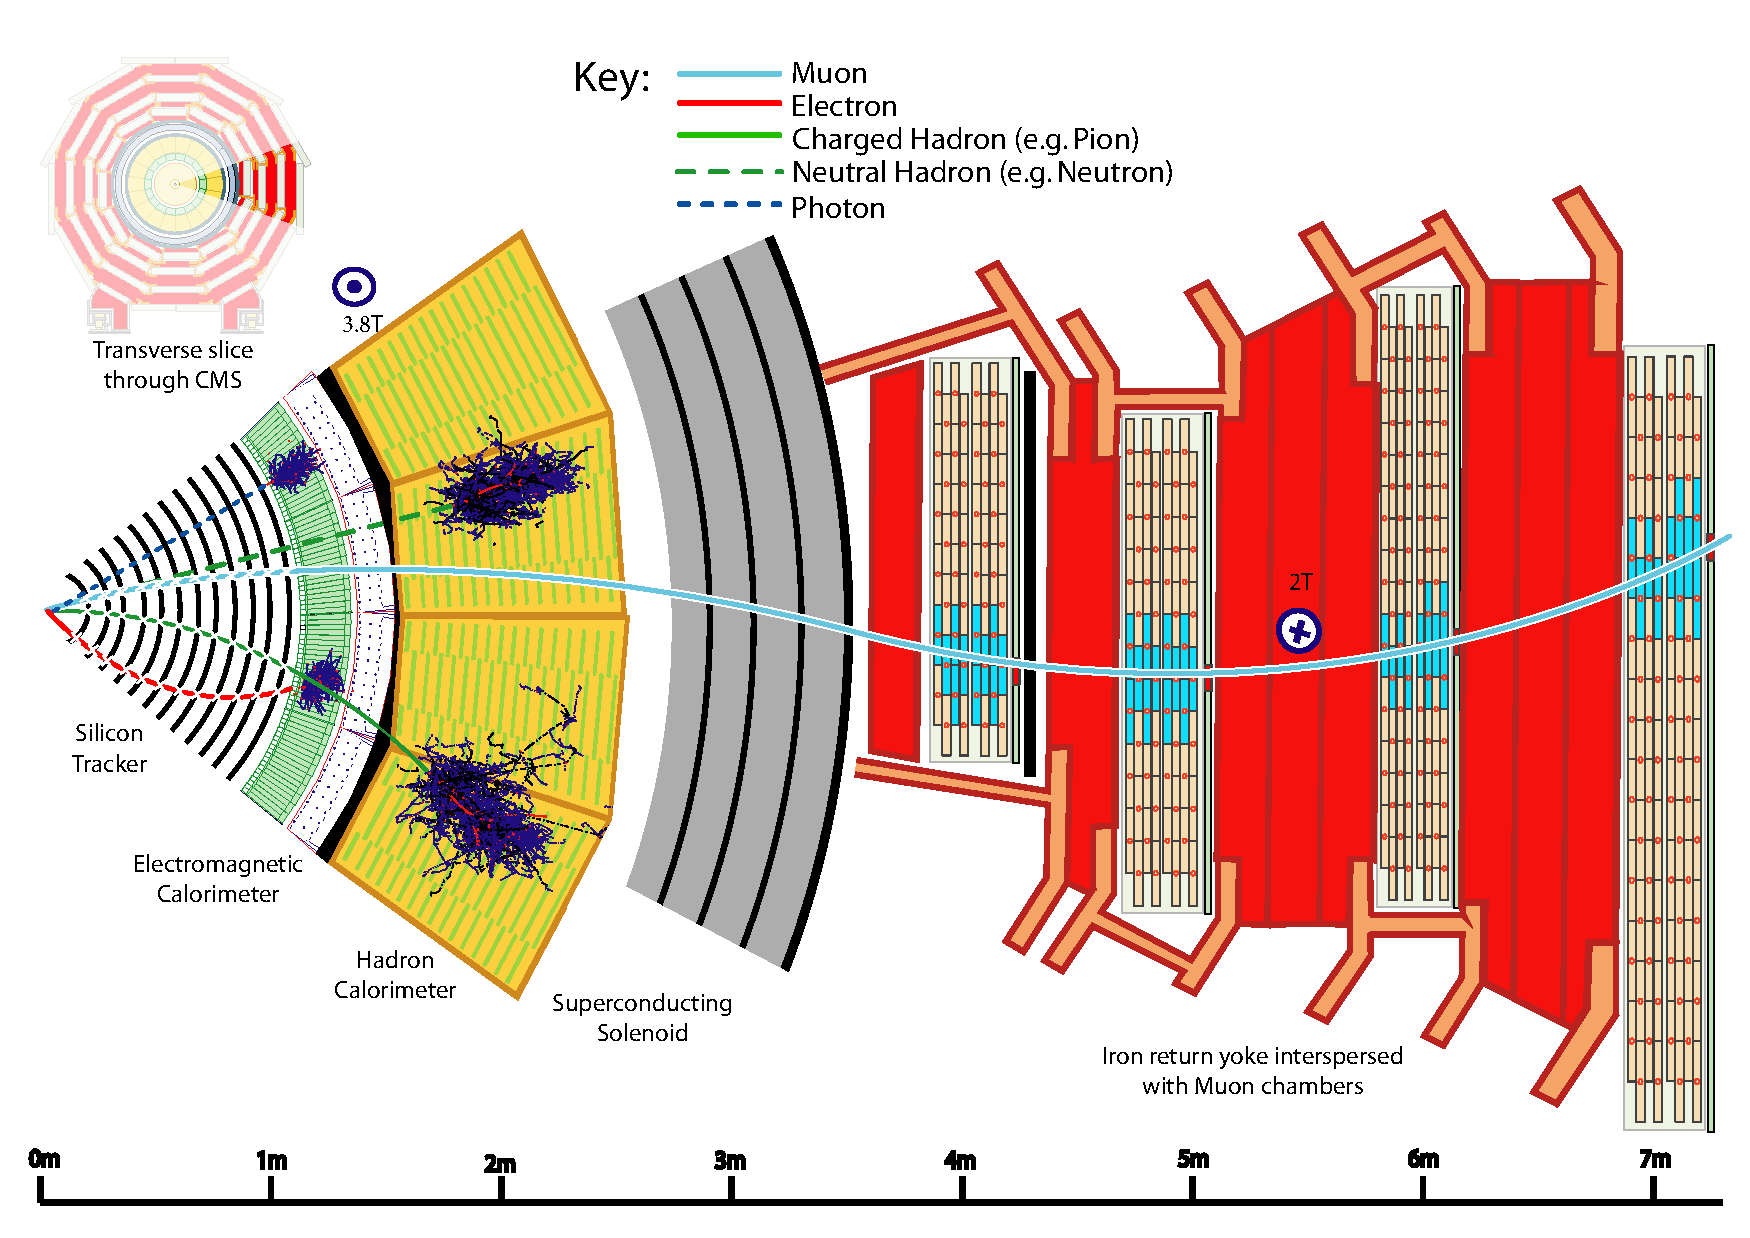
\includegraphics[width=\textwidth]{figures/Reconstruction/CMSDetectorParticleFlow.pdf}
  \caption{
    Idealized picture of particle interactions with the CMS detector subsystems.
        }
 \label{fig:particleFlow}
\end{figure}

When an event is accepted by the HLT, the raw, digitized data from each detector
subsystem is stored and simultaneously forwarded to a commercial processing farm for
further processing. Detector-specific attributes, such as signal amplitudes,
are converted to physical properties, such as energies, using calibrations
established from controlled, independent measurements. System-wide patterns
are built, from which a global picture of the event and its component particles
is extracted.
The reconstruction algorithms employed by the CMS Collaboration are built from
work that began well before the LHC began taking data, 
benefiting from generations of previous experiments. The development of algorithms
is an iterative process, with continual optimizations and incremental changes
being made. The techniques described here relate to the data collection and reconstruction
used by the CMS Collaboration in 2016. Many aspects of the reconstruction
are shared by all analyses performed by the CMS Collaboration. 

A degree of ambiguity in particle identification is unavoidable. 
Reconstruction \emph{efficiency}, or a high rate of positive identification
and reconstruction of real particles, must be balanced alongside the rate of misreconstruction
and misidentification.
For example, electrons with a poorly reconstructed track will mimic photons,
but because the track reconstruction efficiency cannot be 
accepting only very high-quality tracks will lead to the rejection
of real electrons if an interaction in the tracker is not readout.
The optimal balance between efficiency and misidentification is dependent
on the characteristics of the signal and background targeted by a particular
analysis. In addition to the common reconstruction features, the identification 
criteria used in this work are also discussed.

\section{Global event description via particle flow}
The general characteristics of physics object identification outlined
above are ubiquitous amongst past, current, and future collider detector
reconstruction algorithms. Rather than applying these criteria object by
object to select particle candidates of interest, 
the CMS Collaboration implements an ambitious \emph{particle flow} (PF)
algorithm that seeks to reconstruct and identify all objects in an
event as particle candidates. This approach relies on a high-granularity
detector and accurate tracking to connect features of different detector
subsystem, which are combined for more accurate energy, momentum, and
spacial measurements. 

\subsection{Tracks and vertices}
Only energy deposits from charged particles traversing the pixel detector and
strip tracker that exceed a threshold energy (adjustable for each element)
are retained for offline storage. The position of each \emph{hit} is locally
reconstructed from clusters of adjacent pixel or strip elements based
on the relative collected charge in the cluster. 
The efficiency for hits to be reconstructed is over 99\% for active 
channels in both the pixel and strip detectors; approximately 98\%
of pixel channels and 96\% of strip channels were active during 2016 data collection.
The hit position is calculated
in local coordinates of the detector elements before being converted
into a global position with respect to the full CMS detector. The transformation
to global coordinates depends on the relative alignment of the individual tracker
elements and their alignment with respect to the other detector systems.
This is established through in situ measurements of the paths of cosmic rays
to an uncertainty neglible with respect to the intrinsic position resolution 
of the silicon detectors~\cite{Chatrchyan:2014wfa}.

The paths of charged particles through the detector are derived by 
fitting curves to the hits along a possible trajectory. 
The high combinatorics of possible track patterns that can be derived
from the large number of hits arising from high-particle-multiplicity
events is a computational challenge.
To reduce the complexity of pattern identification
while maintaining a high efficiency of reconstruction, the tracking finding
algorithm proceeds in steps, designed to first identify unambiguous
tracks before recovery those of lower quality.
Hits used to form tracks in are removed from consideration in the following
steps, reducing the complexity and chance for misassociation.

In all steps, the algorithm begins with an initial projection of the track
direction, referred to as the track \emph{seed}. The track is then formed
sequentially by extrapolating outward from the beam interaction---in the 
case of tracks seeded by the inner tracker, or inward from seeds in the muon
chambers of calorimeter clusters. Subsequent hits are located 
by predicting their location with using the
Combinatorial Track Finder (CTF) alogrithm~\cite{Chatrchyan:2014fea}, 
an adaptation of the combinatorial Kalman filter algorithm~\cite{Billoir:1989mh}. 
At each step, the projected trajectory is updated to account for the additional
associated seeds, simultaneously building and fitting the particle path.
When the full trajectory through the tracker is established, the track
is refit and discarded if it fails to meet quality criteria, such as 
an excessively high $\chi^{2}$ of the fit.

The first track-forming iterations target high-quality, high-$\pt$ tracks associated
with the beam crossing region, or \emph{beam spot}, established over many
collisions by fitting the expected Gaussian beam profile to the observed
pixel tracks. These initial iterations use seeds formed from hits in each layer of 
the pixel detector, relaxed to two hits in subsequent iterations. 
Following iterations relax the requirement for the track seed to be
compatible with the beam spot, instead seeding via successive hits in the strip
tracker, increasing sensitivity
to displaced tracks from heavy-flavor hadron decays. 
Final iterations are seeded by the muon detectors using an outside-in approach.

Electrons traveling through the tracker have up to $\approx$85\% probability 
of radiating photons (known as bremsstrahlung)
due to interactions with the significant tracker material. Therefore, electron
tracks are likely to exhibit sharp kinks from sudden energy loss by bremsstrahlung.
A modified algorithm known as Gaussian sum filter (GSF)~\cite{Adam:2005bya} is thus employed to 
more accurately reconstruct electron-like tracks. In the CTF algorithm, the
Kalman filter accounts for the material interactions with a Gaussian
smearing around the expected hit location. In the GSF algorithm, 
a sum of Guassian terms, designed to reproduce the Bethe formula for electron
energy loss~\cite{doi:10.1098/rspa.1934.0140}, is used. The GSF algorithm is applied to a subset of 
tracks formed via the CTF algorithm that have few associated hits or a relatively
poor $\chi^{2}$ to obtain an improved description under the electron hypothesis.
The GSF algorithm is also used to form tracks seeded by energy clusters in the 
ECAL, described in Section~\ref{sec:ereco}.

Because the collisions analyzed for this work generally involve multiple $\pp$ interactions,
tracks originate from a variety or vertices. Vertices 
associated with a $\pp$ collision and not an interaction or decay displaced from
the collision point are identified by evaluating the common points of origin for a subset
of the track collection that are well-reconstructed (low $\chi^{2}$) and consistent with
the beam spot. No additional condition on the track $\pt$ is applied
to select this reduced track collection. The deterministic
annealing algorithm~\cite{Rose:726788} is used to group the tracks into their most probably set
of common vertices, before the vertex coordinates are derived by a fit to the 
associated tracks, considering their likelihood of misassignment to the vertex.

The \emph{primary vertex} is the vertex associated with the hard scattering interaction
of interest. The vertex that maximizes $\sum_{i}\pt^{2}$, where the sum considers
the tracks associated with the vertex---clustered using the anti-\kt algorithm
described in Section~\ref{sec:jreco} with radius parameter $R=0.4$---and the 
transverse momentum imbalance associated with the vertex and clustered tracks.
Studies of simulated $\WZ$ events demonstrate that this approach selects the
correct $\pp$ vertex more than 99\% of the time for signal processes considered here. 

\subsection{Muon system tracking}

Charged particles traversing the muon system ionize
the gas, leading to electrical signals on the wires and strips of the
detector systems that are reconstructed as hits. As for the tracker,
the hits are used to infer the paths and momenta of the interacting particles.
All charged objects will be reconstructed by the system, but
the large material presented by the tracker, ECAL, HCAL, and the support
structure and magnet in front of the muon system, ensures that the vast majority
of the objects reaching the system are muons.

Hits in the individual DTs, CSCs, and RPCs are reconstructed using the
principles described in Chapter~\ref{ch:lhcAndCMS}. 
Straight-line tracks, known as ``segments,'' are built by fitting
the hits across each chamber for the CSC and DT subsystems, which
are built from multiple layers of independent gas volumes.
The efficiency for the muon systems to reconstruct hits or segments
from real muons traversing the system is evaluated using the ``tag-and-probe''
technique, for which the momentum and identification of selected
events can be inferred from independent characteristics to calibrate
the detector performance. The hit efficiency of DTs is found to be
greater than 97\% over the entire system; for RPCs, it is greater than
94\% (96\%) in the barrel (endcap).
The trigger requirement for the CSC chambers requires several
consistent tracks, which biases efficiency measurements for individual
hits. The efficiency to reconstruct segments through the chambers is
instead considered. It is evaluated to be 97.4\% efficient for real muons,
determined from the percentage of ``probe'' muons reconstructed in 
the tracker that traverse the CSC detector to those with a reconstructed segment in the CSC chamber.
Groups of DT and CSC segments are used to seed a Kalman-filter based
tracking algorithm that builds ``standalone'' muon tracks from hits 
in the muon system~\cite{Sirunyan:2018fpa}.

\subsection{Calorimeter clusters}
The calorimeters measure both the location of an interacting
electron, photon, or hadron, and its energy. Because energy is deposited
in a shower with a significant depth and transverse extent, the energy
must be collected across several crystals, scintillators, or fibers.
An accurate energy measurement relies on collecting
as close to 100\% of the energy as possible. In addition, the distribution
of the energy deposit in space can be used to identify the particle
that induced the shower.

\emph{clusters} of energy are formed separately for the 
barrel and endcaps of the ECAL and HCAL and the 
ECAL preshower by combining the energy measurements in segmented
components of the detectors. 
Reconstruction is seeded by detector elements with a measured energy deposit
$E>E_{seed}$, from which \emph{superclusters} are formed
by aggregating neighboring detector cells with the seed cell that exceed
energy threshold of twice the noise level. The $E_{seed}$ values are optimized 
independently for the detector regions 
from simulation studies of photons and hadrons.
The values range 
from a few hundred MeV for the ECAL barrel and endcap up to over 1\GeV in the HCAL
endcap; the exact values are given in Table 2 of Ref.~\cite{CMS-PRF-14-001}
Clusters are formed from the superclusters by assuming the energy
deposit from an interaction is Gaussian distributed. The number of interactions
contributing to the supercluster is obtained from a maximum likelihood fit
that considers the number of Gaussian energy deposits and their amplitudes.
In the case of multiple deposits, the distributions obtained from the fit
are used to divide decompose the supercluster into individual clusters.
Because of the rough segmentation in the
forward region, HF clusters consist of a single segmented area.

\subsection{Particle flow candidates}
\label{sec:pfcandidates}

The principle role of the PF algorithm is to \emph{link} the
the inner tracks, muon system tracks, and calorimeter clusters to form 
\emph{PF candidates}. The PF candidates are categorized as neutral or charged
hadrons, electrons, muons, and photons
that are be used in to correct the energy response
of the detector in a particle-specific way and to
build the identified objects selected for analysis. 
The link algorithm evaluates to consistency of tracks and clusters by
extrapolating the from the last hit of each inner track to:
\begin{itemize}
  \item The depth in the ECAL of the expected maximum energy deposit a typical electromagnetic shower
  \item The plane of the ECAL preshower layers
  \item One hadronic interaction length into the HCAL
\end{itemize}
Tracks and clusters are linked if a cluster is found within one
ECAL or HCAL crystal. In the case of multiple matches, the cluster
with its maximum closest to the track position is taken.
Clusters in the ECAL and HCAL are linked if the ECAL clusters overlaps
the HCAL cluster. For GSF tracks linked to an ECAL cluster, 
energy deposits in the ECAL consistent with photon radiation at 
a tangent to the GSF at a silicon layer are collected and linked to the
GSF track and ECAL cluster.

The linked tracks and energy clusters, referred to as \emph{PF blocks},
are further analyzed to be cauterized as a specific particle candidate
that is used in the final selection of events of interest. 
First, muons are identified by linked tracks in the tracker and muon system.
Electrons and photons are then considered simultaneously. Electrons
are seeded by GSF tracks linked to ECAL clusters whereas photons are seeded 
by ECAL clusters with no linked track. Candidates are classified as PF
electrons based on a multivariate regression trained on characteristics
of the GSF track and the energy cluster. The PF photons are categorized
by isolation and the ratio of energy in linked ECAL and HCAL clusters.

For each step, PF blocks associated with PF candidates are removed before
further categorization. After removing muons, electrons, and photons,
remaining blocks are categorized as charged and neutral hadrons.
Neutral hadrons are formed from clusters in the HCAL that are not linked
to ECAL deposts, whereas charged hadrons require an ECAL and HCAL
cluster link. 
The momentum of tracks linked to HCAL clusters is used to improve the poor
resolution of the HCAL for a significant improvement below several hundred GeV.
Because the most ubiquitous neutral hadron, $\pi^{0}$, decays
to two photons, neutral candidates are dominated by photons, which much
better energy resolution than neutral hadrons.
In the HF, the ratio of energy deposits in the long fibers to short fibers
is used to categorize clusters as HF photon and charged hadron candidates.
The PF identification is used to correct the energy assignment based on
object-specific calibrations in the calorimeters.

\section{Physics objects}
\subsection{Muons}
Muons selected for this analysis must be identified as global muons
by the PF algorithm described previously. 
They must be within the muon detector acceptance $\abs{\eta} < 2.4$
and must have $\pt > 10\GeV$. 
Additional reconstruction
criteria are applied to reject \emph{nonprompt} muons, arising 
from hadron decays, and hadron \emph{punch through} into the muon system,
while maintaining a reconstruction efficiency greater than 96\%. 
Following the \emph{Tight} identification criteria of Ref.~\cite{CMS-DP-2017-007},
with slight modifications,
muon candidates must satisfy:

\begin{itemize}
  \item The global muon fit must satisfy $\chi^2/\text{d.o.f.} < 10$ 
    (where d.o.f is the number of degrees of freedom in the fit) 
  \item The distance of the track vertex from the primary vertex in the $x$-$y$
    plane $d_{xy}$ must satisfy $d_{xy} < 0.2\unit{mm}$
  \item The longitudunal distance (in the $z$ plane) of the track vertex from the primary vertex 
    plane $d_{z}$ must satisfy $d_{z} < 1\unit{mm}$
  \item At least one hit in the pixel detector
  \item More than five hits in the strip tracker
  \item At least six hits in the tracker must be used in the track fit.
\end{itemize}

To reject muons from decays of hadrons in jets,
selected muons are required to be isolated from other PF objects
in the event. The relative muon isolation, the ratio of the sum of
the \pt in an $\eta$-$\phi$ region $\Delta R < 0.4$
around the muon is defined as
\begin{equation}
  I_{\mu,rel} = \frac{1}{\pt^{\mu}}\sum_{\Delta R < 0.4}\left[\pt^{h^{\pm,PV}} -  
        \max\left(\pt^{h^{0}}+\pt^{\gamma} - \frac{1}{2}\pt^{h^{\pm, PU}}, 0\right)\right] \,.
\end{equation}
Here $\pt^{h^{\pm,PV}}$ and $\pt^{h^{0}}$ are, respectively, the charged and neutral hadrons
identified by the PF algorithm. The tracks of charged hadron candidates allow them to be
associated to the primary vertex, $h^{\pm,PV}$ or to pileup interactions, $h^{\pm, PU}$.
Such an assignment cannot be made reliably for neutral hadrons and photons, therefore,
all neutral hadrons and are included in the sum. To account for the expected pileup contribution,
the sum is corrected by the term $\pt^{h^{\pm}}/2$, because particle production in 
pileup interactions is expected to be dominated by charged hadron production at nearly this
ratio. A rough estimation of hadron production spit evenly beween $\pi^{+}$, $\pi^{-}$ and $\pi^{0}$ 
gives exactly this ratio, and detailed simulations confirm this expectation.

The $I_{\mu,rel}$ is used to define a baseline, or \emph{loose muon ID}, and
a signal, or \emph{tight muon ID}. Explicitly, the criteria $I_{\mu, rel} < 0.4 (0.15)$
is used for loose (tight) ID. Muons satifying the loose ID, but not the tight ID,
are to estimate the residual contamination from nonprompt muons in the event selection. 
Tight muons are used for to select signal-like events. Further description
of the approach is given in Chapter~\ref{ch:analysis}.

\subsection{Electrons}
\label{sec:ereco}
Electron identification for this analysis begins with the GSF tracks linked
to the ECAL clusters by the PF algorithm. However, unlike for muons,
selected electrons are not uniquely a subset of the PF electrons candidates.
In particular, the BDT discriminant used by the PF algorithm to
categorize electrons and photons is not considered. Instead,
conditional criteria (referred to as ``cuts'') are applied to specific characteristics of the
electron candidate tracks and associated clusters.

Electron candidates must be within the ECAL detector acceptance $\abs{\eta} < 2.5$
and must have $\pt > 10\GeV$. 
As for muons, baseline (\emph{loose}) and \emph{tight} selections is 
are defined. Electrons
satisfying the baseline selection are used to estimate the residual
contribution from nonprompt electrons, while electrons satisfying the both the loose selection
and the full \emph{tight} criteria are selected as signal candidate events in the analysis.
The baseline selection was originally designed to mimic the electron selections applied
at the HLT level for the tightest trigger paths used in this analysis,
however, stronger conditions were applied at the HLT towards the end 
of data collection. Nonetheless, the efficiency loss is recovered by additional
trigger paths as described in Chapter~\ref{ch:analysis}.
The requirements placed on the selected \emph{loose} and \emph{tight} electron
candidates are summarized in Table~\ref{tab:elecID}. The definitions and 
motivations of the variables shown are discussed in the following.

Conditions on the GSF track and linked PF superclusters in the ECAL and HCAL
are applied to select candidates of interest. 
The track and cluster positions must be consistent, defined by a the
variables $\abs{\Delta\eta_{seed}}$ and $\abs{\Delta\phi_{in}}$.
The $\Delta\eta_{seed}$ is the difference between the $\eta$ direction
specified by the track seed and the $\eta$ of the PF cluster that seeds
the ECAL supercluster, and $\Delta\phi_{in}$ is the difference between
the track seed extrapolated to the supercluster and the supercluster $\phi$.
The energy threshold for electron detection ensures that the electron
mass is negligible, so the momentum measured by the track curvature and 
energy measured by the ECAL should be nearly equal. This is ensured by requiring
the variable $1/\pt^{track}-1/E^{SC}$, where $E^{SC}$ is the energy of the supercluster,
be close to zero. Electrons deposit the majority of their energy in the ECAL. 
Therefore, the ratio of the hadronic to electromagnetic energy $H/E$, measured
in terms of the PF ECAL and HCAL clusters, should be small.
To ensure a well-reconstructed track,
the baseline (loose) electron selection requires a good GSF track $\chi^2$.
For the tight identification, the track is required to have at most one
missing hit in the tracker, and the electron candidate is rejected if
any tracks consistent with a photon-to-\EE conversion are found.

The variable $\sigma_{i\eta i\eta}$ is used to assess the shape of the shower
in the $\eta$. It is defined as
\begin{equation}
  \sigma_{i\eta i\eta} = \sqrt{\sum_{i\in 5\times5}\frac{ w_{i}(i\eta_{i} - \bar{i\eta})}{w_i^2}}\,,
\end{equation}
where the sum is over the $5\times5$ block of ECAL crystals centered around the
cluster seed, and the weights $w_i$ are defined as
\begin{equation}
  w_i = \max\left(0, 4.7+\ln{\frac{E_i}{E_{5\times5}}}\right)\,.
\end{equation}
The variable $i\eta_i$ is the $\eta$ of each crystal in the sum,
expressed in integer units numbering the crystals, a choice that allows the variable
gaps between crystals to be ignored. In the endcaps, the arrangement of crystals
is in the $x$-$y$ plane, and $i\eta\def \sqrt{ix^2+iy^2}$ with crystal integer 
numbering $ix$. The $\bar{i\eta}$ is the $i\eta$ of the $5\times5$ cluster,
$E_i$ is the energy of the $i$th crystal, and $E_{5\times5}$ ise the energy 
sum of the $5\times5$ cluster.

As for muons, selected electrons must be isolated from other event activity.
The isolation is defined as 
\begin{equation}
I^{\ell} = \left( \sum  \pt^\text{charged} + \text{max}\left[ 0, \sum \pt^\text{neutral}
                                 +  \sum \pt^{\gamma} - \pt^{\mathrm{PU}}  \right] \right) /  \pt^{\ell}\,,
\end{equation}
where the sum considers objects contained in a cone of $\Delta R < 0.3$ around the electron.
The exact definition depends on the physics objects considered in the sum,
and the approach to pileup subtraction.
For the loose electron selection, the isolation defined in terms of the tracks and
in terms of the PF energy clusters in the ECAL and HCAL are considered separately.
The track isolation considers only charged tracks in the tracker, neglecting the
neutral component and neglecting corrections for the isolation.
For the PF cluster isolations, the
sum of ECAL and HCAL cluster energies 
are corrected by estimated the pileup energy contribution per event using the 
``jet area'' technique proposed for jets in Ref.~\cite{Cacciari:2007fd}.
In this approach,
$\pt^{\mathrm{PU}} \equiv \rho \, A_\text{eff}$,
where the average transverse momentum $\rho$ is calculated from
the median of the ratio of the jet transverse momentum to the jet area, $\pt^{\jet}/A_{\jet}$,
for all pileup jets in the event.
The effective area $ A_\text{eff}$ is the geometric area of the isolation 
cone times an $\eta$-dependent correction factor
that accounts for the residual dependence of the isolation on the pileup.
The $A_\text{eff}$ is calculated separately for the terms (e.g., neutral or charged)
considered in the pileup subtraction.
For the tight electron identification criteria, the PF objects are used. Charged PF candidates
are required to be associated with the primary vertex. Because the neutral objects cannot be
directly associated with a vertex, so the pileup correction considers only the neutral
component.

\begin{table}[htbp]
    \centering
    \caption[Identification criteria for selected electrons]{
      The identification criteria used to select electrons for used to estimate
      nonprompt backgrounds (loose ID) and to select signal events (tight ID).
      The variable of interest specified in the leftmost column must be smaller
      than the values indicated to the right. The conditions on the barrel region
      ($\abs{\eta} < 1.479$) and the endcap ($1.479 < \abs{\eta} < 2.5$) are optimized
      independently.
            }
    \begin{tabular}{lcccc} 
                        & \multicolumn{2}{c}{Loose ID} & \multicolumn{2}{c}{Tight ID}  \\
      Variable                & ECAL barrel & ECAL endcap & ECAL barrel & ECAL endcap        \\
    \hline
      $\abs{\Delta\eta_{seed}}$ & 0.004     & ---         & 0.00308     & 0.0605 \\
      $\abs{\Delta\phi_{in}}$   & 0.020     & ---         & 0.0816      & 0.0394 \\
      $\abs{E_{SC}^{-1} - p_{track}^{-1}}$  & \multicolumn{2}{c}{0.013} & 0.0129 & 0.0129 \\
      $\sigma_{i\eta i\eta}$  & 0.011       & 0.031       & 0.00998     & 0.0298 \\
      $H/E$                   & 0.060     & 0.065       & 0.0414      & 0.0641 \\
      $I^{ECAL}$        & 0.160     & 0.120       & \multicolumn{2}{c}{1} \\
      $I^{HCAL}$        & \multicolumn{2}{c}{0.120} & \multicolumn{2}{c}{1} \\
      $I^{track}$       & \multicolumn{2}{c}{0.08} & \multicolumn{2}{c}{1} \\
      $I_{e,rel}^{PF,corr}$     & \multicolumn{2}{c}{---} & 0.0588      & 0.0571 \\
      GSF track $\chi^{2}/\text{d.o.f.}$  & ---                     & 3.0         & \multicolumn{2}{c}{---} \\
      Max missing tracker hits  & \multicolumn{2}{c}{---} & \multicolumn{2}{c}{1} \\
    \hline 
     \end{tabular}
    \label{tab:elecID}
\end{table}

\subsection{Jets}
\label{sec:jreco}
As introduced in Chapter~\ref{ch:phenomenology} and discussed
in Chapter~\ref{ch:simulation}, partons produced in the hard interaction
are observed in the detector as clusters of hadronized particles known
as jets. Perturbative predictions rely on a clustering algorithm that
is insensitive to the low-angle and low-energy behaviour of partons. 
A variety of such ``infrared-safe'' algorithms have been developed
and studied; an overview can be found in Ref.~\cite{Salam:2009jx}.
Because it is advantageous to use a common jet-clustering algorithm for experimental
measurements and theoretical predictions, the anti-$\kt$ algorithm~\cite{Cacciari:2008gp}
is used by both the ATLAS and CMS Collaboration.

The anti-$\kt$ algorithm sequentially clusters objects into composite jets
based on their separation in rapidity $y$ and azimuthal angle $phi$. A weighted distance
parameter is defined by
\begin{equation}
  d_{ij} = \min(k_{\text{T}i}^{-2}, k_{\text{T}j}^{-2})\frac{\Delta R^2_{ij}}{R^2}\,.
\end{equation}
where $R$ is the radius parameter, $k_{\text{T}i}$ and $k_{\text{T}j}$ index the transverse momentum of the objects considered
in the comparison, and $\Delta R^2 = (y_i - y_j)^2 + (\phi_i-\phi_j)^2$.
A parameter $d_{iB} = k_{\text{T}i}^2$ is defined as the $\pt$ of the $i$th object
with respect to the beamline.
The values of $d_{ij}$ and $d_{iB}$ are computed for all objects in the event.
If a value $d_{ij}$ is the minimum parameter, the $i$th and $j$th objects are
merged into a composite objects by summing the four vectors. If $d_{iB}$ is
the minimum, the object is removed from further iterations. The procedure
is repeated until all objects in the event are clustered.

The anti-$\kt$ algorithm has several favorable theoretical and experimental properties: it is infrared safe,
results in a jet that is circular in the $y$-$\phi$ plane for hard partons $i$ and $j$ with
$\Delta R_{ij} > 2R$, and is computationally fast in the 
\texttt{FastJet}~\cite{Cacciari:2011ma} implementation.
A radius parameter of $R=0.4$ is used for this analysis. This is the choice made by 
the majority of 13\TeV studies made by the ATLAS and CMS Collaborations,
as it is found to be
a good balance between minimizing the jet size to reduce contributions from pileup
and maximizing the jet size to capture all hadrons associated with the fragmentation
of hard partons.

Selected jets used in this analysis are defined by clustering the PF
candidates reconstructed in Section~\ref{sec:pfcandidates}. To reduce the contributions
from pileup, charged hadrons unambiguously not associated to the primary vertex
are removed from the PF candidates collection before clustering~\cite{CMS-PAS-JME-14-001}
(referred to as charged-hadron subtracted, or CHS jets). 
Leptons are not removed from the subset of PF candidates considered,
however, clustered jets with $\Delta R(\jet, \ell) < 0.4$ are removed from the jet collection.
The contribution from neutral pileup is subtracted from the jet energy using the jet area method
described for lepton isolation. 

The energy scale and resolution of the jets is corrected in data and simulation 
to account for the complex detector response and inefficiencies. 
The detector response is nonlinear and dependent on the jet composition,
which may not be well-modeled by MC simulations, so the energy corrections
are derived and applied to the clustered jets rather than the individual PF constituents.
The corrections are primarily derived from MC simulation, using ratios
of ``generator'' jets formed by clustering all stable ($c\tau > 1\unit{m}$) 
hadronized particles in the MC simulation to jets of PF CHS jets in the reconstructed simulation.
The ratios are used to correct the energy of reconstructed jets in the MC simulation
and in data. Residual differences in data and MC simulations are corrected for by
measuring the jet energies in data and MC for samples of $\Zpj$, $\gamma+$jet,
and dijet events. For single jet events, the energy of the $\PZ$ bosons (with decays to electrons or muons)
or $\gamma$ should be balanced with the momentum of the recoiling jet.
For dijet events, a well-measured jet in the central part of the detector
is balanced with a forward jet to derive energy corrections in the region
beyond the tracker acceptance~\cite{Khachatryan:2016kdb}. 

\begin{figure}[htbp]
  \centering
   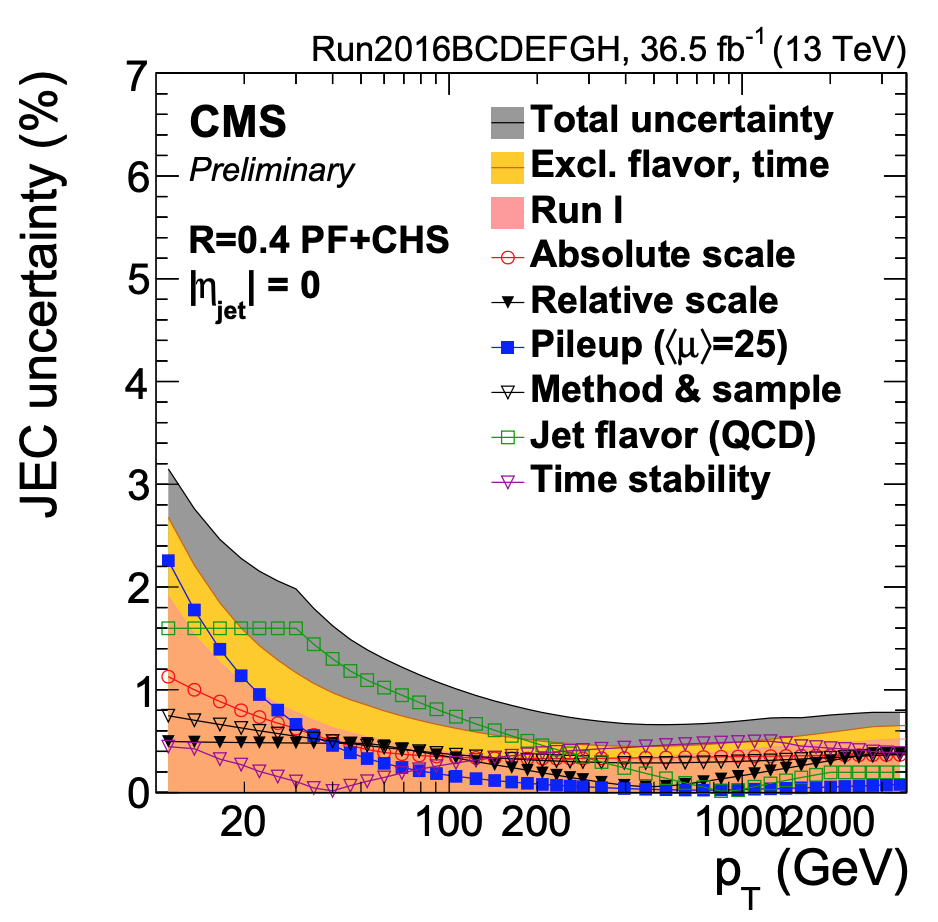
\includegraphics[width=0.49\textwidth]{figures/Reconstruction/JECUncertaintyEta.png}
   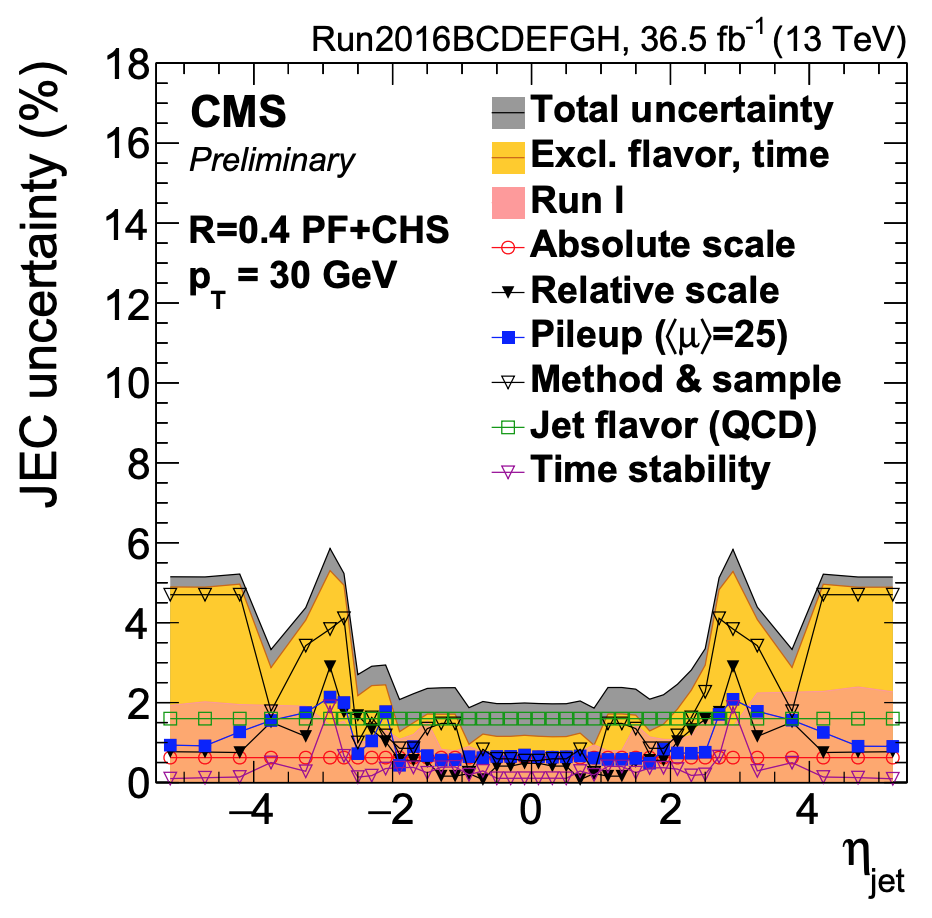
\includegraphics[width=0.49\textwidth]{figures/Reconstruction/JECUncertaintyPt.png}
  \caption[The uncertainty in the jet energy corrections vs. jet $\eta$ and $\pt$]{
    The uncertainty in the jet energy corrections (JEC) for PF charged-haron-subtracked (CHS) jets
    vs. jet $\pt$ (left) and jet $\eta$ (right) for fixed
    jet $\pt=30\GeV$. The total uncertainty and the uncertainty by component of the
    energy correction type are shown.
        }
 \label{fig:jecUnc}
\end{figure}

The uncertainty in the procedure is estimated by assessing the uncertainty
in each component of correction, including comparisons
of the residual corrections in data and MC simulation with different data samples and 
variations of the pileup subtracting estimation~\cite{CMS-DP-2018-028}. The total uncertainty and 
the uncertainty by correction component are shown in Fig.~\ref{fig:jecUnc}.
As illustrated, the uncertainty increases at high $\eta$ to 5-6\% for $\pt=30\GeV$ jets.
Because forward jets are a key component of this analysis, the jet energy
scale and resolution uncertainties are the leading contributions to the measurement uncertainty.

\subsection{Heavy-flavor jets}

The hadronization of $\cPqb$ quarks primarily produces
baryons and mesons with larger masses and lifetimes
than pions or other first- and second-generation hadrons. The 
decay lengths of such B-hadrons (e.g., B$^{0}$, a $\cPqd\cPaqb$ bound state) 
produced at the LHC are typically on the order of
centimeters~\cite{Tanabashi:2018oca}. The decay products of such B hadrons
will be dispaced from the primary vertex by this amount, which is within
the resolution of the track reconstruction to be distinguished from the primary
vertex. This observation is exploited to distinguish jets arising from the 
hadronization of $\cPqb$-quarks. Because the branching ratio 
$\mathcal{BR}(t\to\PW\cPqb)~1$, b-quark tagging is an effective means to identify
top-quark production, a major background for this analysis.

The $\cPqb$ quark jets are identified in this analysis via
the combined secondary vertex \cPqb-tagging algorithm~\cite{Chatrchyan:2012jua} with the 
\textit{tight} working point defined in Ref.~\cite{Sirunyan:2017ezt}. 
The algorithm using information on the PF candidate tracks and their
associated vertices in the jet to train a multivariate discriminant,
which is trained to distinguish b hadrons in MC simulation.
The efficiency for selecting {\cPqb} quark jets 
with $\pt>30\GeV$ and $\abs{\eta} < 2.4$
with the tight working point is $\approx$49\% with
a misidentification probability of $\approx$4\% for {\cPqc} 
quark jets and $\approx$0.1\% for light-quark and gluon jets.

\subsection{Missing transverse momentum}

Neutrinos produced in the hard scattering interaction are inferred
from the total imbalance in transverse momentum of the event,
referred to as the \emph{missing transverse momentum} $\ptvecmiss$.
It is reconstructed from the sum of all the PF candidates
in the event,
\begin{equation}
  \ptvecmiss = - \sum_{\text{PF cands}} \vec{p}_{T,cand}\,.
\end{equation}
Pileup collisions, which are generally soft hadronic interactions,
do not produce significant $\ptvecmiss$. Therefore, all PF candidates
in the event are used in the sum, even those not associated with
the primary vertex. 

The measurement of the $\ptvecmiss$ is improved by correcting
jet energies with the procedure described in the previous section. 
The PF candidates that are clustered into jets are subtracted from
the $\ptvecmiss$ sum and replaced by the corrected energies,
\begin{equation}
  \vec{p}_{T,corr}^{\kern1pt\text{miss}} = \ptvecmiss - 
        \left(\pt^{\jet} - \sum_{\text{cand}\in\jet} \vec{p}_{T,cand}\right)\,.
\end{equation}
The uncertainty in the corrected $\ptmiss$, used for this analysis, is dominated by the uncertainty in the 
jet energy corrections. A smaller uncertainty is associated with the
\emph{unclustered energy} of PF candidates not associated with a jet~\cite{Sirunyan:2019kia}.

Spurious $\ptvecmiss$ arises in events in which an object is significantly
mismeasured, biasing the momentum sum of the event. Events with 
features of detector noise, such as large spikes in a
single ECAL crystal or HCAL readout, as well as those with muon interactions
in the calorimeters and CSC chambers that are symmetric in $\phi$, indicative
of $\emph{beam halo}$ muons produce in proton beam interactions with the 
beam pipe material, are vetoed. 

Because the $\eta$ direction of the $\ptvecmiss$ vector is unknown,
its magnitude $\ptmiss$ is generally considered. In this analysis,
the $\ptmiss$ is used to select events with a tectonically decaying $\PW$
boson giving rise to $\ptmiss\sim m_{\PW}/2$.
